
\begin{itemframe}{الگوریتم جانسون}
\itm
الگوریتم جانسون
\fn{Johnson Algorithm}
مانند الگوریتم فلوید وارشال برای یافتن کوتاه ترین مسیر بین هر دو راس گراف است. این الگوریتم برای گراف‌های خلوت پبچیدگی زمانی کمتری نسبت به بقیه روش‌ها (فلوید وارشال و روش شبیه‌سازی ضرب ماترسی) دارد.

\itm
الگوریتم جانسون -مانند الگوریتم بلمن فورد- می‌تواند روی گراف دارای یال منفی کوتاه ترین مسیر را به درستی محاسبه کند و وجود دور منفی در گراف را تشخیص و گزارش دهد. (گراف دارای دور منفی در مسئله کوتاه ترین مسیر یک حالت خطا محسوب می‌شود.)
%todo number of this footnote is not correct
\footnote{برای گراف دارای دور منفی یافتن کوتاه ترین مسیر ساده می‌تواند کاربرد داشته‌باشد. این مسئله ان‌پی-سخت است.}
\end{itemframe}


\begin{itemframe}{الگوریتم جانسون}
\itm
برای طراحی یک الگوریتم مسئله کوتاه‌ترین مسیر بین هر جفت رأس می‌توان V بار اجرا کردن یکی از الگوریتم‌های کوتاه‌ترین مسیرهای هم مبداء را به عنوان یک حد بالا برای مرتبه زمانی تحلیل کرد.

\itm
برای مثال
$|V|$
بار اجرای الگوریتم بلمن فورد مرتبه
$O(V^2E)$
و
$|V|$
بار اجرای الگوریتم دایجسترا مرتبه
$O(VE+V^2lgV)$
را به دست می‌دهد.
\itm
روش دوم سریع‌تر است امّا در گراف‌‌هایی که یال منفی داشته باشند به درستی کار نمی‌کند.
\end{itemframe}


\begin{itemframe}{الگوریتم جانسون}
\itm
الگوریتم جانسون نیز از ایده‌ایی مشابه استفاده می‌کند. این الگوریتم هر دو الگوریتم بلمن-فورد و دایجسترا را فراخوانی می‌کند؛
\item[۱]
جانسون در مرحله اول، الگوریتم بلمن-فورد را استفاده می‌کند تا وجود دور منفی را تشخیص دهد و در صورتی که دور منفی وجود داشت آن را گزارش داده و کار تمام می‌شود.
\item[۲]
در صورتی که دور منفی وجود نداشت، این الگوریتم با استفاده از روشی که در ادامه بررسی خواهد شد، همه وزن‌ها را به مقادیر غیر منفی نگاشت می‌کند.
\item[۳]
حال که همه وزن‌‌های غیر منفی شده‌اند برای هر رأس یک بار الگوریتم دایجسترا اجرا می‌شود تا کوتاه ترین مسیرها از هر رأس به بقیه رئوس محاسبه شوند.
\end{itemframe}


\begin{itemframe}{الگوریتم جانسون}
\itm
اما چطور باید وزن‌های گراف را به مقادیر غیر منفی نگاشت کرد؟ واضح است که بعد از تغییر وزن‌ها نباید کوتاه ترین مسیرها را تغییر کنند. برای مثال اضافه کردن یک مقدار ثابت به همه وزن‌ها نگاشت مناسبی نیست. برای درک بهتر این موضوع به مثال زیر توجه کنید:
\begin{center}
	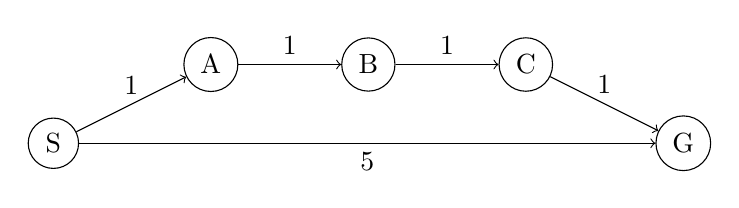
\begin{tikzpicture}[->]
		\node[circle,draw] (S) at (0,0) {S};
		\node[circle,draw] (G) at (8,0) {G};
		\node[circle,draw] (A) at (2,1) {A};
		\node[circle,draw] (B) at (4,1) {B};
		\node[circle,draw] (C) at (6,1) {C};

		\draw (S) -- node[below] {5} (G);
		\draw (S) -- node[above] {1} (A);
		\draw (A) -- node[above] {1} (B);
		\draw (B) -- node[above] {1} (C);
		\draw (C) -- node[above] {1} (G);
	\end{tikzpicture}
\end{center}
\itm
اضافه کردن یک واحد به همه یال‌ها کوتاه ترین مسیر از S به G را تغییر می‌دهد:

\begin{center}
	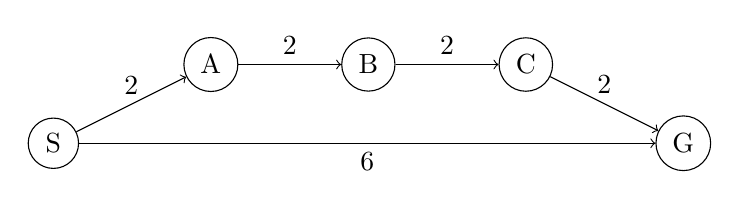
\begin{tikzpicture}[->]
		\node[circle,draw] (S) at (0,0) {S};
		\node[circle,draw] (G) at (8,0) {G};
		\node[circle,draw] (A) at (2,1) {A};
		\node[circle,draw] (B) at (4,1) {B};
		\node[circle,draw] (C) at (6,1) {C};

		\draw (S) -- node[below] {6} (G);
		\draw (S) -- node[above] {2} (A);
		\draw (A) -- node[above] {2} (B);
		\draw (B) -- node[above] {2} (C);
		\draw (C) -- node[above] {2} (G);
	\end{tikzpicture}
\end{center}
\end{itemframe}


\begin{itemframe}{الگوریتم جانسون}
\itm
بیایید ویژگی‌های این تغییر وزن را به طور دقیق‌تر بررسی کنیم؛\\
فرض کنید وزن‌های گراف توسط تابعی به نام «تابع وزن»
\fn{weight function}
داده شده. به طوری که وزن یال بین u و v برابر است با
$w(u, v)$.
آنگاه تابع وزن جدیدی مانند
$\hat{w}$
باید این دو ویژگی را داشته باشد:
\item[1]
به ازای هر
$u, v \in E$
مسیری مانند p با استفاده از تابع وزن
$w$
یک کوتاه ترین مسیر از u به v است اگر و تنها اگر مسیر p با استفاده از تابع وزن
$\hat{w}$
نیز یک کوتاه ترین مسیر باشد.
\item[2]
به ازای هر
$u, v \in E$
مقدار
$\hat{w(u, v)}$
غیر منفی باشد.
\end{itemframe}


\begin{itemframe}{الگوریتم جانسون}
\itm
الگوریتم جانسون از این تغییر وزن استفاده می‌کند:
\begin{align*}
\hat{w(u, v)} = \m{w(u, v)} + h(u) - h(v)
\end{align*}
\itm
به طوری که u رأس شروع و v رأس پایان یال است و h تابعی است که به هر رأس یک عدد حقیقی نسبت می‌دهد.
\itm
در ادامه ثابت خواهیم کرد که این تغییر وزن به ازای هر تابع h کوتاه‌ترین مسیرها را تغییر نمی‌دهد اما برای تبدیل همه وزن‌ها به مقادیر غیر منفی، تابع h باید به درستی تعریف شود.
\end{itemframe}


\begin{itemframe}{الگوریتم جانسون}
\itm
ابتدا باید ثابت ‌کنیم رابطه تغییر وزن ارائه شده ویژگی اول را ارضاء می‌کند.
\itm
فرض کنید
$ p= \langle v_0, v_1, ..., v_k \rangle$
یک مسیر از
$v_0$
به
$v_k$
باشد. همچنین وزن کل مسیر p با تابع وزن w را با  w(p) نشان می‌دهیم. آنگاه
$\hat{w}$
برابر است با:
\begin{align*}
\hat{w(p)= (\hat{w}(v_0, v_1) + h(v_0) -  h(v_1)) + (\hat{w}(v_1, v_2) + h(v_1) -  h(v_2)) + } \\
(\hat{w}(v_2, v_3) + h(v_2) -  h(v_3)) + ... + (\hat{w}(v_{k-1}, v_k) + h(v_{k-1}) -  h(v_k))
\end{align*}

\end{itemframe}


\begin{itemframe}{الگوریتم جانسون}
\itm
رابطه بالا نشان می‌دهد برای هر رأس مثل u، مقدار h(u) به وزن یک یال اضافه می‌شود و از یال بعدی کسر می‌شود (به غیر از رأس ابتدا و انتهای مسیر). بعد از ساده‌سازی به این رابطه می‌رسیم:
$$\hat{w}(p)=w(p) + h(h(v_0) - h(v_k)$$
\itm
بنابراین برای هر دو رأس مشخص به همه کوتاه‌ترین مسیرهای بین آن دو رأس یک مقدار ثابت اضافه می‌شود پس این نگاشت وزن کوتاه ترین مسیرها را تغییر نمی‌دهد.
\end{itemframe}

\begin{itemframe}{الگوریتم جانسون}
\itm
هدف بعدی این است که شرایطی فراهم کنیم که ویژگی دوم هم برقرار باشد. برای این کار یک رأس جدید به نام s به گراف اضافه می‌کنیم. سپس این رأس را با یال‌هایی با وزن صفر به همه رئوس دیگر متصل می‌کنیم به طوری که یال ‌ها از s خارج شوند.
\centerimg[.4]{figs/shortest-path/4.png}
شکل بالا نمونه‌ایی از این تغییر را نشان می‌دهد (رأس آبی رنگ به گراف اضافه شده‌است).
\end{itemframe}


\begin{itemframe}{الگوریتم جانسون}
\itm
سپس تعریف می‌کنیم مقدار h برای هر رأس مثل v برابر است با کوتاه ترین مسیر از s به v . در شکل بالا نیز اعداد نوشته‌شده بر رأس‌ها به همین طریق محاسبه شده‌اند.
\itm
حال با استفاده از نامساوی مثلثاتی می‌دانیم که به ازای هر

$(u, v \in E)$
رابطه زیر برقرار است:
$$
h(v) \leqslant h(u)+w(u, v)
$$
\itm
اگر رابطه بالا برقرار نباشد نتیجه می‌شود که مسیر h(v) کوتاه‌ترین مسیر نبوده و به تناقض می‌رسیم.
\itm
سپس h(u) را به سمت راست نامساوی می‌بریم:
$$
0\leqslant w(u, v) + h(u) - h(v)
$$
\itm
سمت راست این نامساوی همان رابطه‌ایی است که برای $\hat{w}$ تعریف شد. بنابراین ثابت شد که به ازای هر
$(u, v \in E)$
مقدار $\hat{w}$ غیر منفی است.
\end{itemframe}


\begin{itemframe}{الگوریتم جانسون}
\itm
درستی الگوریتم جانسون ثابت شد. شکل زیر یک نمونه از گراف تغییر وزن یافته توسط الگوریتم جانسون است:
\centerimg[.3]{figs/shortest-path/5.png}

\itm
قبلا اشاره شد که الگوریتم جانسون از الگوریتم بلمن-فورد برای تشخیص دور منفی استفاده می‌کند. همچنین دیدم که برای محاسبه تابع h نیاز به مقادیر کوتاه‌ترین مسیر از s به بقیه رئوس نیاز داریم. می‌دانیم الگوریتم بلمن-فورد توانایی محاسبه هر دوی این موارد را دارد. بنابراین الگوریتم جانسون با یک بار اجرای بلمن-فورد هم کوتاه‌ترین مسیرها از s را محاسبه می‌کند و هم وجود دور منفی را تشخیص می‌دهد.
\end{itemframe}


\begin{itemframe}{الگوریتم جانسون}
\itm
برای یافتن وزن اصلی یک مسیر از رابطه زیر استفاده می‌کنیم:
$$
w(p(u, v)) = \hat{w}(p(u, v)) + h(v) - h(u)
$$
\itm
در نهایت به تحیلی پیچیدگی زمانی الگوریتم جانسون می‌پردازیم:
\itm
اجرای $|V|$ بار الگوریتم دایجسترا زمان‌برترین مرحله الگوریتم جانسون است بنابراین -مانند دایجسترا- باید گراف را در لیست مجاورتی ذخیره کنیم. حال اگر فرض کنیم الگوریتم دایجسترا با استفاده از هرم فیبوناچی پیاده‌سازی شده‌است، پیچیدگی زمانی برابر است با
$O(V^2lgV+VE)$
که از ضرب یک
$|V|$
در مرتبه زمانی دایجسترا به دست آمده‌است.
\itm
در صورتی که گراف خلوت باشد مرتبه زمانی این الگوریتم برابر است
$O(V^2lgV)$.
در حالی که الگوریتم فلوید-وارشال برای گراف خلوت از مربته زمانی
$O(V^3)$
است.
\end{itemframe}